\subsubsection{Der Cocktailmixer}\label{subsubsec:Der_Cocktailmixer}
\paragraph{Aufbau}\label{subsubsec:Aufbau_Der_Cocktailmixer}\mbox{}\\

Der Cocktailmixer ist ein 1m breites und 76cm hohes Küchengerät auf Rollen. Im Unterschrank können bis zu 28 Zutaten gelagert werden. Das Gehäuse besteht aus Edelstahl und ist sehr aufwendig und professionell gestaltet, sodass es in einer Restaurantküche einen Platz finden könnte. Die Schläuche führen im Schrank zum Flüssigkeitsauslass und sind bei geschlossenen Fronttüren nicht sichtbar. Gemäss Hersteller können 14-40 Getränkeanschlüsse realisiert werden. Die Behälter haben standardmässig ein Volumen von 5 Liter und können bei Bedarf auch auf 10 und 20 Liter erweitert werden. Über der Oberfläche befindet sich ein einziger Flüssigkeitsauslass. Die Maschine kann in der bestehenden Theke eingebaut werden. Gesteuert wird die Maschine von einer SPS-Steuerung, welche eine hohe Verlässlichkeit ohne Ausfällen gewährleisten soll.\cite{bg_innovation_cocktailmaschine_nodate}

\paragraph{Bedienung}\label{subsubsec:Bedienung_Der_Cocktailmixer}\mbox{}\\

Die Bedienung geschieht mittels einem 7’’ Touch-Display, welches sich über dem Flüssigkeitsauslass befindet. Das selbe Display wird auch in der Schifffahrt gebraucht und ist deswegen besonders robust und Flüssigkeitsresistent.\cite{bg_innovation_cocktailmaschine_nodate}

\paragraph{Technische Daten}\label{subsubsec:Technische_Daten_Der_Cocktailmixer}\mbox{}\\

\begin{tabular}{@{}llp{0.6\textwidth}}
    Zeit für einen Cocktail: & : & Für die Zubereitung eines Cocktails benötigt die Maschine lediglich   3-5 Sekunden. Somit sind bis zu 300 Cocktails in der Stunde möglich. \cite{bg_innovation_cocktailmaschine_nodate}\\
    \hline
    Anzahl verschiedene Cocktails: & : & Abhängig von der Anzahl Getränkeanschlüssen können mehr oder weniger Getränke zubereitet werden. Der Speicherplatz bietet jedoch Platz für 500 gespeicherte Cocktails. Die Cocktails können frei programmiert und gespeichert werden, genauso wie die Dosierungseinstellungen. Dies kann direkt an der Maschine vorgenommen werden und benötigt keiner Software. \cite{bg_innovation_cocktailmaschine_nodate}\\ 
    \hline
    Stromversorgung: & : & Der Cocktailmixer benötigt in jedem Fall einen Festanschluss an das Stromnetz. \cite{bg_innovation_cocktailmaschine_nodate}\\
\end{tabular}

\paragraph{Reinigung}\label{subsubsec:Reinigung_Der_Cocktailmixer}\mbox{}\\

Über die Reinigung wurden keine Angaben gefunden.

\paragraph{Sonstiges}\label{subsubsec:Sonstiges_Der_Cocktailmixer}\mbox{}\\

Die Erweiterung der Flüssigkeiten und Pumpen kann jeweils in Zweierschritten geschehen. In den für die Flüssigkeiten vorgesehenen Behältern ist eine Füllstanderkennung eingebaut. Der Support ist sehr ausführlich, es gibt Schulungen in der Software der Cocktailmaschine und die Maschine wird inklusive An- und Abfahrt aufgebaut. Das verwendete Material, worin die Getränke gelagert werden, sind lebensmittelzertifiziert.\cite{bg_innovation_cocktailmaschine_nodate}

\begin{figure}[h]
	\centering
	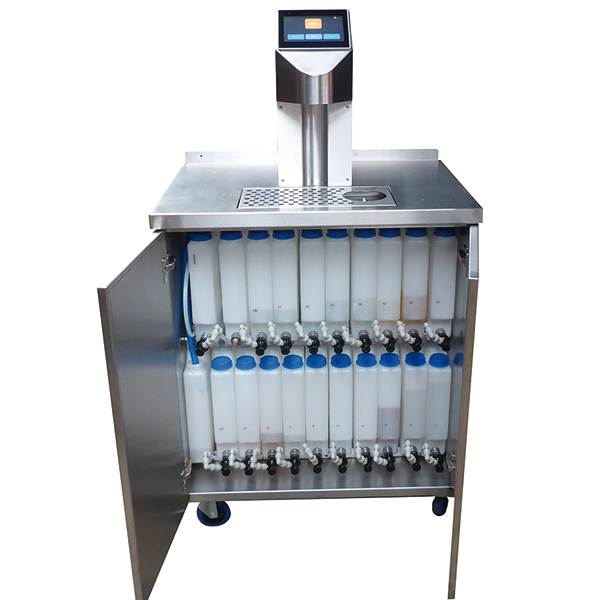
\includegraphics[width=0.4\textwidth]{graphics/DerCocktailmixer.png}
	\caption{Der Cocktailmixer \cite{bg_innovation_cocktailmaschine_nodate}}
	\label{fig:DerCocktailmixer_Cocktailmaschine}
\end{figure}